\documentclass[tikz,convert={outfile=fonctions.png}]{standalone}

    \usepackage[utf8]{inputenc}

\begin{document}
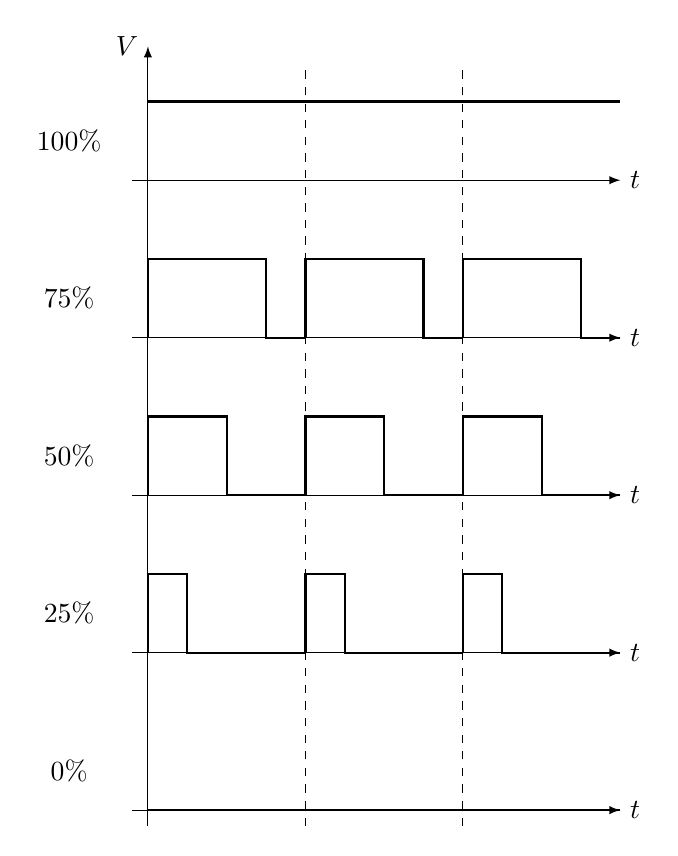
\begin{tikzpicture}[>=latex]

    \foreach \i in{0,...,4}{
        \draw[->] (-.2,\i*2) -- ++(6.2,0) node[right] {$t$};
    }
    %\draw[->] (0,\i*2-.2) -- ++(0,1.7) node[left] {$V$};
    \draw[->] (0,-.2) -- (0,9.7) node[left] {$V$};
    \draw[dashed] (2,-.2) -- (2,9.5);
    \draw[dashed] (4,-.2) -- (4,9.5);

    % signal 0%
    \foreach \i in {0,...,2} {
        \draw[thick] (\i*2,0) -- ++(2,0);
    }

    % signal 25%
    \foreach \i in {0,...,2} {
        \draw[thick] (\i*2,2) -- ++(0,1) -- ++(0.5,0) -- ++(0,-1) -- ++(1.5,0);
    }

    % signal 50%
    \foreach \i in {0,...,2} {
        \draw[thick] (\i*2,4) -- ++(0,1) -- ++(1,0) -- ++(0,-1) -- ++(1,0);
    }

    % signal 75%
    \foreach \i in {0,...,2} {
        \draw[thick] (\i*2,6) -- ++(0,1) -- ++(1.5,0) -- ++(0,-1) -- ++(.5,0);
    }

    % signal 75%
    \foreach \i in {0,...,2} {
        \draw[thick] (\i*2,9) -- ++(2,0) ;
    }
    \draw (-1,0.5) node {0\%};
    \draw (-1,2.5) node {25\%};
    \draw (-1,4.5) node {50\%};
    \draw (-1,6.5) node {75\%};
    \draw (-1,8.5) node {100\%};

\end{tikzpicture}
\end{document}

